\documentclass[landscape, headrule, footrule]{foils}
\usepackage{amsmath, amssymb, amsfonts, theorem, plain}
\usepackage{lscape}
\usepackage{caption2}
\usepackage{floatflt}
\usepackage{wrapfig}
\usepackage[below]{placeins}
\usepackage{fancybox}
\usepackage[pdftex]{geometry}
\geometry{headsep= 0.2in, footskip=0.2in, hscale=0.9}

\usepackage{pifont}

\usepackage{subfigure}
\usepackage[pdftex, usenames]{color}  %for colors
\usepackage[pdftex]{graphicx}     %for importing graphics
\usepackage{times}  %for nice fonts

\usepackage{background} % only work for ppower4
\usepackage{pp4slide}   % only work for ppower4
\usepackage{pause}      % only work for ppower4
\usepackage{mpmulti}    % only work for ppower4

\usepackage[pagebackref]{hyperref} %for hyperlinking and other pdf effects


\makeatletter
\newcommand{\figcaption}{\def{\@captype}{figure}\caption}
\newcommand{\tabcaption}{\def{\@captype}{table}\caption}
\makeatother


\newcommand{\gb}[1]{\ensuremath{\boldsymbol{#1}}}
\newcommand{\ve}[2][\ensuremath{x}]{\ensuremath{(#1_1, \ldots, #1_{#2})}}

\definecolor{DarkGreen}{rgb}{0.5,0.8,0.6}
\definecolor{RGBblack}{rgb}{0.0,0.0,0.0} 
\vpagecolor[blue]{RGBblack} % it's command in \usepackage{background} but only work for ppower4

\hypersetup{
  pdftitle={PDF and Web (from Latex) and Miscellaneous},
  pdfsubject={How to post LaTeX work to Web?},
  pdfauthor={Eugenia Yu and Weiliang Qiu,
    Department of Statistics,
    University of British Columbia},
  pdfkeywords={Web, HTML, PDF, hyperref, LaTeX, Conversion, DOC, gvim},
  pdfpagemode={FullScreen},  %make the pdf start in full-screen mode
  %pdfpagemode={None},
  linkcolor=cyan,  %make all the links cyan instead of red
  citecolor=cyan,  % color for bibligraphical citations in text.
  pagecolor=cyan,  % color for links to other pages.
  urlcolor=cyan,    % color for linked URLs.
}


\rightfooter{\NavigationBar}

\providecommand{\NavigationBar}{{\Large
  \Acrobatmenu{PrevPage}{\reflectbox{\ding{227}}}
  \Acrobatmenu{NextPage}{\ding{227}}
  \Acrobatmenu{FirstPage}{\reflectbox{\ding{224}}}
  \Acrobatmenu{LastPage}{\ding{224}}
  \Acrobatmenu{GoBack}{\reflectbox{\ding{249}}}
  \Acrobatmenu{Quit}{\ding{54}}%
}}



\leftheader{PDF and Web (from Latex) and Miscellaneous}
                                            %make a left header
%\rightheader{\textsf{\thepage}}            %make a right header
\MyLogo{Eugenia and Weiliang, UBC Stats}    %make a left footer
%\rightfooter{}                             %make a right footer


\title{\shadowbox{PDF and Web (from Latex) and Miscellaneous}} % the document title

% the author
\author{Latex Smart \\
         6356 Agricultural Road\\
         University of British Columbia\\
         Vancouver BC \\
         V6T 1Z2}

% the date
\date{\today}

\begin{document}

\thispagestyle{empty}

\setcounter{page}{0}
\maketitle

\foilhead[-0.5in]{Outline}
\LogoOn
\hypersetup{pdfpagetransition=Dissolve}
\begin{itemize}
  \item The Web, its documents, and \LaTeX
  \item Conversion between formats (latex, dvi, pdf, ps, html, Word docs)

  \item Revisit \LaTeX\, macro \verb+\def, \newcommand+ and \verb+\renewcommand+

  \item Editors (e.g. gvim, emacs and winedit)

  \item rejoinder 
\end{itemize}

%\foilhead[-0.5in]{Why do we need to translate \LaTeX\, to HTML?}


\foilhead{Ways to publish \LaTeX\, document into Web}
\hypersetup{pdfpagetransition={None}}
\MyLogo{Eugenia and Weiliang, UBC Stats}    %make a left footer
\begin{itemize}
  \item Generate \textsc{postscript} or \textsc{dvi} files and add hyperlinks to these files. 
    \begin{description}
      \item[pros] easy to do and convenient for authors. 
      \item[cons] \quad
\begin{itemize}
  \item may be inconvenient for readers. Readers need to download these files to local disk and 
need viewers (e.g. ghostview, xdvi) to view the files.

  \item cannot show hyperlinks for ps files\footnote{\texttt{xdvi} supports the loading of a Web
browser when a URL link is encountered, but it cannot be integrated within a Web browser.}.
\end{itemize}
    \end{description}
\end{itemize}

\foilhead[-0.8in]{Ways to publish \LaTeX\, document into Web (Ct'd)}
\begin{itemize}
  \item Generate \textsc{pdf} file. 
    \begin{description}
      \item[pros] \quad
\begin{itemize}
  \item easy to do and convenient for authors
  \item can easily navigate through the document and exploit hypertext information that might be
present in the \LaTeX\, source.
  \item don't need to download files to local disk.
  Web browsers can be configured to load Acrobat as a helper. Acrobat can also pass URL links to
the browser with a seamless integration.
  \item has the ability to render pages with layout essentially exactly as in an original 
(e.g. \LaTeX) document.
\end{itemize}
      \item[cons]\quad
\begin{itemize}
  \item ``A helper or plug-in has to be installed on the viewing system''.
  \item ``It restricts searchability because the document is not text''. 
  \item ``It requires a verbose and bulky file format that includes all the non-standard 
fonts that are used''\cite{GoossensEtAl:1999}.
\end{itemize}
    \end{description}
\end{itemize}


\foilhead{Ways to publish \LaTeX\, document into Web (Ct'd)}
\begin{itemize}
  \item Translate \LaTeX\, into HTML.
  \item Use Java and browser plug-ins to display a \LaTeX\, source directly inside a browser. 
\end{itemize}

%\rotatefoilhead[-0.5in]{Similarity between \LaTeX\, and HTML}
%\MyLogo{The table is from p. 11, \cite{GoossensEtAl:1999}}    %make a left footer
%\begin{center}
%{\tiny
%\begin{tabular}{lll}
%\hline
%\textit{Description} & \textsc{html} & \LaTeX\, equivalent\\
%\hline
%\multicolumn{3}{c}{\textit{Document sectioning commands}}\\
%\hline
%\textit{level 1} & \verb+<H1>text</H1>+ & \verb+\chapter{text}+\\
%\textit{level 2} & \verb+<H2>text</H2>+ & \verb+\section{text}+\\
%\textit{level 3} & \verb+<H3>text</H3>+ & \verb+\subsection{text}+\\
%\textit{level 4} & \verb+<H4>text</H4>+ & \verb+\subsubsection{text}+\\
%\textit{level 5} & \verb+<H5>text</H5>+ & \verb+\paragraph{text}+\\
%\textit{level 6} & \verb+<H6>text</H6>+ & \verb+\subparagraph{text}+\\
%\textit{new paragraph} & \verb+<P>+ & \verb+\par+\\
%\hline
%\multicolumn{3}{c}{\textit{Highlighting text}}\\
%\hline
%\textit{emphasis} & \verb+<EM>text</EM>+ & \verb+\emph{text}+\\
%\textit{bold font} & \verb+<B>text</B>+ & \verb+\textbf{text}+ (\verb+\mathbf{text}+)\\
%\textit{teletype font} & \verb+<TT>text</TT>+ & \verb+\texttt{text}+ (\verb+\mathtt{text}+)\\
%\hline
%\multicolumn{3}{c}{\textit{Lists}}\\
%\hline
%\textit{ordered list} & \verb+<OL>...</OL>+ & \verb+\begin{enumerate}...\end{enumerate}+\\
%\textit{unordered list} & \verb+<UL>...</UL>+ & \verb+\begin{itemize}...\end{itemize}+\\
%\textit{list term} & \verb+<LI>text+ & \verb+\item text+\\
%\textit{description list} & \verb+<DL>...</DL>+ & \verb+\begin{description}...\end{description}+\\
%\textit{description term} & \verb+<DT>text+ & \verb+\item[term]+\\
%\textit{description data} & \verb+<DD>text+ & \verb+text+\\
%\hline
%\multicolumn{3}{c}{\textit{Special characters}}\\
%\hline
%\textit{accents (e.g., \'e)} & \verb+&eacute;+ & \verb+\'e+\\
%\textit{umlauts (e.g., \"u)} & \verb+&uuml;+ & \verb+\"u+\\
%\textit{newline} & \verb+<BR>+ & \verb+\newline+\\
%\hline
%\end{tabular}
%The table is from p. 11 of \cite{GoossensEtAl:1999}.
%}
%\end{center}
%

\foilhead[-0.5in]{What are difficulties to do the translation?}
\MyLogo{This slide is from \cite{Hutchinson}.}
\begin{itemize}
  \item \TeX\, is capable of extremely detailed page layout, specifying precisely where on the page symbols go.
HTML is not, because HTML is a functional mark-up language (specifying primarily document structure) not a page layout language.

  \item HTML's exact rendering is not specified by the document that is published but is, to some degree, left to the discretion of the browser.

  \item \TeX's excellent mathematical capabilities are absent from HTML and browsers. 

  %\item If you require your readers to see an exact replication of what your document looks like to you, then you cannot use HTML to transmit it, no matter what format it starts in.
\end{itemize}

\foilhead[-0.5in]{Two main choices for representing equations in HTML}
\begin{itemize}
  \item using bit-mapped images
    \begin{description}
      \item[pros] it uses capabilities that are essentially universal to every graphical
browser.
      \item[cons] \quad
\begin{itemize}
  \item it requires a separate graphical file for every equation, which becomes very
cumbersome and slow to download.

  \item also the alignment and sizing of the graphical equations is uncertain with respect to the rest of the text.
\end{itemize}
    \end{description}

Software: \texttt{LaTeX2HTML}, \texttt{TeX4ht}.


  \item using browser fonts and tables for layout
    \begin{description}
      \item[pros] one HTML document contains all the information, giving portability and speed of
download. 
      \item[cons] it depends on having the symbol font accessible on the browser, and that the equation layout 
is not as compact or elegant as \TeX's.
    \end{description}

Software: \texttt{TtH}.

\end{itemize}


%\foilhead[-0.5in]{LaTeX2HTML}

%\foilhead[-0.5in]{TeX4ht}

\foilhead[-0.5in]{Direct display of \LaTeX\, on the web}
\MyLogo{Eugenia and Weiliang, UBC Stats}    %make a left footer
\begin{itemize}
  \item Using browser plug-in, such as \texttt{techexplorer}.
\begin{description}
  \item[pros] \quad
\begin{itemize}
  \item understands a large subset of the \LaTeX.
  \item fast
\end{itemize}
  \item[cons]\quad
\begin{itemize}
  \item the plug-in must be downloaded and installed on all browsers you want to use.
  \item a separate version of the plug-in is needed for each computer platform.
\end{itemize}
\end{description}
\end{itemize}

\foilhead[-0.5in]{Direct display of \LaTeX\, on the web (Ct'd)}
\begin{itemize}
  \item Using Java applets, such as \texttt{WebEQ}.
\begin{description}
  \item[pros]\quad
\begin{itemize}
  \item produce good quality display
  \item can adapt to resizing of the browser window size and fonts.
\end{itemize}

  \item[cons] \quad
\begin{itemize}
  \item slow
  \item does not strictly process \LaTeX, but rather a variant called WebTeX.
\end{itemize}
\end{description}
\end{itemize}

%\rotatefoilhead[-0.8in]{Suggestions Given by Goossens et al.}
%\begin{quote}
%\begin{itemize}
%  \item Is it purely text, and straightforward \LaTeX? Then translate it directly into HTML (for
%instance, with \texttt{TtH}), or start preparing to work in \texttt{XML}.
%  \item Does it contain lots of low-level math with homegrown macros that allow you to set up
%your own customized notation? Then you would probably use TeX4ht or \LaTeX2HTML (in the latter
%case, be prepared to write some Perl scripts implementing your extensions) or if you prefer
%a commercial solution, use MicroPress' VTEX.
%  \item Does it contain lots of ``normal'' math? Envision translating that into MathML, and use
%one of the browser plug-ins.
%  \item Does it use a lot of non-Latin characters? You would probably want to use a
%\LaTeX-to-XML converter and translate the non-Latin characters into Unicode.
%  \item Does it have a complex layout (tables, perhaps) or typography that is essential to the
%document reader? Use \textsc{pdf}.
%  \item Is your document fairly self-contained? Do you have little interaction with other Web
%material? Consider an approach based on \textsc{dvi}.
%\end{itemize}
%\end{quote}
%

\foilhead[-0.5in]{The \texttt{hyperref} package}
\begin{itemize}
  \item it extends the functionality of all the \LaTeX\, cross-referencing commands (including
the table of contents, bibliographies, and so on).
  \item it also provides new commands to allow the user to write ad hoc hypertext links,
including those to external documents and URLs.
  \item it should be the \textbf{last} of the loaded package in case its commands being
overwritten.
  %\item If the \texttt{implicit} option is set to \texttt{false}, then only explicit hyperlink
%commands will be processed and all cross-references will not be preocessed.
%\begin{verbatim}
%  \usepackage[implicit=false]{hyperref}
%\end{verbatim}

\end{itemize}


\foilhead[-0.5in]{Configuring \texttt{hyperref}}

The syntax
\begin{verbatim}
  \hypersetup{keyvalue pairs}
\end{verbatim}

Example:
\begin{verbatim}
\hypersetup{
  pdftoolbar=true,
  pdfmenubar=true,
  pdffitwindow=true,
  pdfpagelayout=TwoColumnLeft 
}
\end{verbatim}

\texttt{TwoColumnLeft} means displaying the pages in two columns ,with odd-numbered pages on the
left.

\foilhead[-0.5in]{Commonly used options of \texttt{hyperref}}
{\small
\begin{tabular}{llll}
\hline
\textit{Option}&\textit{Value}&\textit{Default}&\textit{Description}\\
\hline
breaklines& boolean& false & Allows link text to break across lines.\\
implicit & boolean& true & Allows to produce hyperlink for all cross-references.\\
\hline
backref & boolean&false & Adds backlink text to the end of each\\
        &        &      & item in the bibliography as a
list of section numbers.\\
pagebackref&boolean&false&Adds backlink text to the end of each item in \\
           &       &      &the bibliography as a
list of page numbers.\\
colorlink&boolean&false&Colors the text of links and anchors.\\
linkcolor&color&red&Color for simple internal links (cross-references).\\
anchorcolor&color&black&Color for anchor text.\\
citecolor&color&green&Color for bibliographical citations in text.\\
pagecolor&color&red&Color for links to other pages.\\
urlcolor&color&cyan&Color for linked network URLs.\\
\hline
bookmarks&boolean&false&Write a set of Acrobat bookmarks, \\
         &       &     &in a manner similar to the table of contents.\\
{\tiny bookmarksopen}&boolean&false&If Acrobat bookmarks are requested,\\
             &       &     & show them with all the subtrees expanded.\\
{\tiny bookmarksnumbered}&boolean&false&If Acrobat bookmarks are requested,\\
             &       &     & include the section numbers.\\
\hline
\end{tabular}
}

\foilhead[-0.5in]{Commonly used options of \texttt{hyperref} (Ct'd)}
{\small
\begin{tabular}{llll}
\hline
\textit{Option}&\textit{Value}&\textit{Default}&\textit{Description}\\
\hline
pdfpagemode &name&None&Determine how the file is opened in Acrobat;\\
            &     &   &the possibilities are \texttt{None, UseThumbs},\\
            &     &   &\texttt{UseOutlines} and \texttt{FullScreen}\\
{pdfpagelayout} & name &SinglePage& Possible values: \texttt{OneColumn},
\texttt{TwoColumnLeft}\\
            &     &    & and \texttt{TwoColumnRight}.\\
\hline
pdftitle &text& &Sets the document information Title field.\\
pdfauthor &text& &Sets the document information Author field.\\
pdfsubject &text& &Sets the document information Subject field.\\
pdfkeywords &text& &Sets the document information Keywords field.\\
\hline
{\tiny pdfpagetransition} &name& &The effect used when going to a new page;\\
\hline
\end{tabular}
}

\foilhead[-0.5in]{Acrobat page transition options}
\begin{table}[ht]
\caption{Acrobat page transition options}
\label{transition}
{
\begin{tabular}{lll}
\hline
\textit{Option}&\textit{Key(s)}&\textit{Description}\\
\hline
Split&\verb+/Dm, /M+ & Two lines sweep across the screen to \\
     &               & show the new page.\\
Blinds&\verb+/Dm+& Multiple lines synchronously sweep in \\
     &           & the same direction.\\
Box &\verb+/M+& A box sweeps from the center out or \\
    &         & from the edges in.\\
Wipe &\verb+/Di+& A single line sweeps across the screen \\
     &          &from one edge to the other.\\
Dissolve&& { The page image dissolves in a piecemeal fashion}.\\
%%Glitter&\verb+/Di+&{ Similar to Dissolve}.\\
\hline
\end{tabular}
}
\begin{itemize}
  \item {It seems that any word other than the above 6 options
will produce normal display.}
  \item Example: \verb+\hypersetup{pdfpagetransition={Blinds /Dm /V}}+. 
\end{itemize}


\end{table}
\foilhead[-0.5in]{Acrobat page transition options (Ct'd)}
{
\begin{description}
  \item[/Di] (Direction) The direction of movement, in degrees (counterclockwise). Values are
generally in $90^o$ steps.
  \item[/Dm] (Dimension) If a choice between horizontal or vertical is allowed, value is
/H (horizontal) or /V (vertical).
  \item[/M] (Motion) If an effect can be from the center out or from the edges in, value is
/I (in) or /O (out).
\end{description}
}


\foilhead[-0.5in]{Hyperlinks}
\hypersetup{pdfpagetransition={Split /Dm /V}}

\shadowbox{\verb+\href{url}{text}+} make a hyperlink to the webpage with address \texttt{url}.

Example: 
\begin{verbatim}
\href{http://www.stat.ubc.ca/~webmaste/howto/
  editor/latex.html#doublespace}{Howto set 
  double space effect in LaTeX}
\end{verbatim}
\href{http://www.stat.ubc.ca/~webmaste/howto/editor/latex.html#doublespace}
{Howto set double space effect in LaTeX}

In \texttt{url}, the special characters \verb+#+ and \verb+~+ do \textbf{not} need to be escaped
in any way.

Note: The effect of this page is by
\begin{verbatim}
\hypersetup{pdfpagetransition={Split /Dm /V}}
\end{verbatim}

\foilhead[-0.5in]{Hyperlinks (Ct'd)}
\hypersetup{pdfpagetransition={Blinds /Dm /H}}

\shadowbox{\verb+\hyperlink{name}{text1}+}\, make a hyperlink to a hypertext object defined
somewhere by \verb+\hypertarget+.

Example:
\begin{verbatim}
\hyperlink{target}{Definition of \texttt{hypertarget}}
\end{verbatim}
\hyperlink{target}{Definition of \texttt{hypertarget}}

Note: The effect of this page is by
\begin{verbatim}
\hypersetup{pdfpagetransition={Blinds /Dm /H}}
\end{verbatim}

\foilhead[-0.5in]{Hyperlinks (Ct'd)}
\hypersetup{pdfpagetransition={Box /M /I}}

\shadowbox{\verb+\hypertarget{name}{text2}+}\, defines a hypertext object. The \texttt{text2} is
not necessarily the same as the \texttt{text1} in \verb+\hyperlink{name}{text1}+. However, the
\texttt{name} in \verb+\hypertarget{name}{text2}+ should be the same as that in
\verb+\hyperlink{name}{text1}+.

Example:
\begin{verbatim}
\hypertarget{target}{}
\end{verbatim}
\hypertarget{target}{}

Note: The effect of this page is by
\begin{verbatim}
\hypersetup{pdfpagetransition={Box /M /I}}
\end{verbatim}

\foilhead[-0.5in]{Hyperlinks (Ct'd)}
\hypersetup{pdfpagetransition={Wipe /Di 90}}

\shadowbox{\verb+\hyperref{label}{text}+}\, make a hyperlink to a point established with a 
normal \LaTeX\, \verb+\label+ command with the symbolic name \texttt{label}.

Example:
\begin{verbatim}
\hyperref[eq1]{This links to Equation (\ref*{eq1}).}
\end{verbatim}

\hyperref[eq1]{This links to Equation (\ref*{eq1}).}

Note: 
\begin{itemize}
  \item \verb+\ref*{eq1}+ generates the right number but not to form a link.

  \item The effect of this page is by
\begin{verbatim}
\hypersetup{pdfpagetransition={Wipe /Di 90}}
\end{verbatim}
\end{itemize}


\foilhead[-0.5in]{Hyperlinks (Ct'd)}
\hypersetup{pdfpagetransition={Dissolve}}

This is the equation referred by the hyperlink defined in the previous page
\verb+\hyperref[eq1]{This links to Equation (\ref*{eq1}).}+:
\begin{eqnarray}\label{eq1}
\int_{a}^{b}x dx=\frac{b^2-a^2}{2}
\end{eqnarray}

  The effect of this page is by
\begin{verbatim}
\hypersetup{pdfpagetransition={Dissolve}}
\end{verbatim}

\foilhead[-0.8in]{\shadowbox{pagebackref}}
\begin{enumerate}
  \item Type \verb+\usepackage[pagebackref]{hyperref}+ in the preamble of the \LaTeX\, file.
  \item Type just before \verb+\end{document}+
\begin{verbatim}
\bibliographystyle{plain}
\bibliography{workshop}
\end{verbatim}
(Suppose the file \verb+workshop.bib+ is in the current directory.)
  \item Use the command \verb+\cite+ to cite reference defined in \verb+workshop.bib+.
Here we cite \cite{GoossensEtAl:1999} (\verb+\cite{GoossensEtAl:1999}+).
\end{enumerate}

\foilhead[-0.8in]{\shadowbox{pagebackref (Ct'd)}}
\begin{itemize}
  \item If there are more than two places referring to the same reference, use option 
\texttt{pagebackref} instead of \texttt{backref} since \texttt{backref} can generate only one
back hyperlink.
  \item If there are some pages with \verb+\thispagestyle{empty}+, then \texttt{pagebackref} will go
back to wrong page.

  \item The effect of this page is by
\begin{verbatim}
%\hypersetup{pdfpagetransition={Dissolve}}
\end{verbatim}
\end{itemize}


\foilhead[-0.8in]{\shadowbox{Acrobatmenu}}
\hypersetup{pdfpagetransition={None}}
The navigation hyperlinks are constructed by adding the following in the preamble:
\begin{verbatim}
\usepackage{pifont}
\rightfooter{\NavigationBar}
\newcommand{\NavigationBar}{{\Large
  \Acrobatmenu{PrevPage}{\reflectbox{\ding{227}}}
  \Acrobatmenu{NextPage}{\ding{227}}
  \Acrobatmenu{FirstPage}{\reflectbox{\ding{224}}}
  \Acrobatmenu{LastPage}{\ding{224}}
  \Acrobatmenu{GoBack}{\reflectbox{\ding{249}}}
  \Acrobatmenu{Quit}{\ding{54}}%
}}
\end{verbatim}

If you have graphics for the navigation bars, you can replace Dingbat with graphic buttons, e.g.

\verb+\Acrobatmenu{NextPage}{\includegraphics{nextpic}}+.

\foilhead[-0.5in]{Conversion between formats}
\begin{center}
\includegraphics[height=1.2\textheight,angle=-90]{conversion}
\end{center}



\foilhead[-0.5in]{Conversion between formats (Ct'd)}
{\small
\begin{center}
\begin{tabular}{l|l|l|l}
\hline
Conversion & Software & free of charge? & available from dept?\\
\hline
  \LaTeX\, $\Rightarrow$ \textsc{dvi}  & latex & free & Yes\\
  \LaTeX\, $\Rightarrow$ \textsc{pdf}  & pdflatex & free & Yes\\ 
  \LaTeX\, $\Rightarrow$ \textsc{html}  & latex2html& free & Yes\\ 
  \LaTeX\, $\Rightarrow$ \textsc{word docs}  & Word2Tex & \$\$ & No\\ 
  \textsc{word docs} $\Rightarrow$ \LaTeX   & Tex2Word & \$\$ & No\\ 
  \textsc{HTML} $\Rightarrow$ \LaTeX   & html2latex & free & No\\ 
  \textsc{dvi} $\Rightarrow$ \textsc{ps} & dvips & free & Yes\\
  \textsc{dvi} $\Rightarrow$ \textsc{pdf} & dvipdfm & free  & Yes\\
  \textsc{ps} $\Rightarrow$ \textsc{pdf} & ps2pdf & free  & Yes\\
  \textsc{pdf} $\Rightarrow$ \textsc{ps} & pdf2ps & free  & Yes\\
  \textsc{pdf} $\Rightarrow$ \textsc{word docs} & Drake Plugin Software & \$\$  & No\\
  \textsc{word docs} $\Rightarrow$ \textsc{pdf} & BCL easy\textsc{pdf} $3.0$ OR & \$\$  & No\\
  & Adobe Acrobat & \$\$  & Yes\\
  \textsc{html} $\Rightarrow$ \textsc{pdf} & Adobe Acrobat & \$\$  & Yes\\
  \textsc{pdf} $\Rightarrow$ \textsc{html} & Intra\textsc{pdf}~.~com & \$\$  & No\\
  various conversions to & \textsc{pdf}995 & free & No\\ 
  and from \textsc{pdf} & & & \\ 
\hline
\end{tabular}
\end{center}
}
\foilhead[-0.5in]{\shadowbox{\texttt{def, newcommand} and
\texttt{renewcommand}}}
\verb+\def+, \verb+\newcommand+, and \verb+\renewcommand+ are used to define
or redefine \LaTeX\, command. The usages are:
\begin{verbatim}
\def{cmd}{def}
\newcommand{cmd}[args][opt]{def}
\renewcommand{cmd}[args][opt]{def}
\end{verbatim}
\begin{description}
  \item[\texttt{cmd}] The name of the new or redefined command. The first
character of \texttt{cmd} must be \verb+\+.
  \item[\texttt{args}] An integer from 1 to 9 denoting the number of
arguments of the command being defined.
  \item[\texttt{opt}] Default value for the first argument.
  \item[\texttt{def}] The definition of the command. Use $\#n$ to denote the
$n$-th argument.
\end{description}


\foilhead[-0.5in]{\shadowbox{\texttt{def, newcommand} and
\texttt{renewcommand} (Ct'd)}}
Example:
\begin{verbatim}
\usepackage{amsmath, amssymb, amsfonts}
\newcommand{\gb}[1]{\ensuremath{\boldsymbol{#1}}}
\newcommand{\ve}[2][\ensuremath{x}]
    {\ensuremath{(#1_1, \ldots, #1_{#2})}}
\end{verbatim}
The command \qquad\verb|$\gb{\alpha} \ve{n}+\ve[y]{n}$|
\qquad produces

\fbox{$\gb{\alpha} \ve{n}+\ve[y]{n}$}.

\foilhead[-0.5in]{\shadowbox{\texttt{def, newcommand} and
\texttt{renewcommand} (Ct'd)}}
\begin{itemize}
  \item For \verb+\newcommand+, \texttt{cmd} must \textbf{not} be already
defined.
  \item For \verb+\renewcommand+, \texttt{cmd} must already be defined.
  \item \verb+\ensuremath+ makes sure its argument be always processed in
math mode.
\end{itemize}

\foilhead[-0.5in]{Editors}
The choice of editor for tex/latex makes a big difference in time
  saving (for both inputs and making changes).

Recommended editors:
\begin{itemize}
  \item \texttt{gVim} with special menus.
  \item \texttt{Emacs} with \textsc{auctex}, \textsc{lightning completion}
and \textsc{ultra-tex}.

  \item \texttt{WinEdit} [Windows shareware only]
\end{itemize}


%\foilhead[-0.5in]{Vi editor}
%\begin{itemize}
%  \item \texttt{Vi} is a Visual Editor. The name Vi is for Visual. Visual editors are ones that let you see multiple lines of
%    the document that you are editing as you edit it. 
%  \item \textsc{vim} stands for ``VI IMproved''.
%  \item \texttt{gVim} operates in a \textsc{gui} (Graphical User Interface) environment. 
%\end{itemize}
%
%\foilhead[-0.8in]{Vi editor (Ct'd)}
%\begin{itemize}
%  \item vi editor has two modes (\texttt{command} mode and \texttt{insert} mode). In the \texttt{command} mode, 
%you can input commands. In the
%    \texttt{insert} mode, you can edit files. To enter into \texttt{command} mode, 
%type \textsc{esc} key. To enter into \texttt{insert} mode from
%    \texttt{command} mode, type character \texttt{i}. 
%  \item Some useful \texttt{gVim} commands:
%    \begin{description}
%      \item[u] undo
%      \item[ctrl+r] redo
%      \item[ctrl+v] define visual block
%      \item[\%] --- to match braket pair (\verb+(,), [,], {,}+). 
%      \item[:!\textit{cmd}] execute a single unix command \textit{cmd}
%      \item[:sh] escape to shell
%      \item[ctrl+w+s] --- to split the current window horizontally.
%      \item[ctrl+w+v] --- to split the current window vertically.
%      \item[ctrl+w+q] --- to close the current window 
%      \item[:10,30s/hello/hi/g] --- to replace ``\textit{hello}'' with ``\textit{hi}'' from $10$-th line
%to $30$-th line.
%    \end{description} 
%\end{itemize}


\foilhead[-0.3in]{\texttt{Vi} (Visual editor) key mapping}
Key mapping is used to change the meaning of typed keys.

Syntax:
\begin{center}
:map lhs rhs
\end{center}

For example:
\begin{verbatim}
      map ,l :!latex %
      map ,b :!bibtex %<  
      map ,s :!dvips -o %<.ps %<.dvi  
      map ,x :!xdvi %<.dvi & 
      map ,p :!pdflatex % & 
      map ,f :!xpdf %<.pdf & 
      map ,a :!acroread %<.pdf & 
      map ,g :!ghostview  %<.ps &
\end{verbatim}


\foilhead[-0.3in]{\texttt{Vi} (Visual editor) key mapping (Ct'd)}
\begin{itemize}
  \item ``\verb+map ,l :!latex %+'' means that map command ``\verb+:!latex %+'' to ``\verb+,l+''.
When you type ``\verb+,l+'', gVim will replace it to the command ``\verb+:!latex %+''.

  \item ``\verb+:!latex %+'' means executing unix command \verb+latex filename+ where
\verb+filename+ is the latex file ``\verb+filename.tex+'' you are editing by using gVim.
  \item You can define the mapping in the file \texttt{.vimrc} in your home directory.
  \item To delete mapping, use \texttt{unmap}. The syntax is \verb+unmap lhs+.
For example \verb+unmap ,l+.
\end{itemize}

\foilhead[-0.8in]{Abbreviations in gVim}
You can define abbreviations in gVim. When you type the abbreviations, gVim will replace the
abbreviation with the complete phrase it stands for. 

Syntax:
\begin{center}
:ab lhs rhs
\end{center}

For example:
\begin{verbatim}
:ab iid independent and identically distributed
:ab wlog without loss of generality
\end{verbatim}
When you type \texttt{iid} and \texttt{space} key, gVim will automatically replace
\texttt{iid} with \texttt{independent and identically distributed}.

To delete abbreviations, use \texttt{una}. The syntax is \verb+una lhs+. For example,
\verb+:una iid+.


\foilhead{Transform a table to LaTeX format by gVim}
\MyLogo{The example is taken from Mark Robinson's Informal Computing Seminar - January 20, 2000}    %make a left footer

You want to transform:  
\begin{verbatim}
0.41 -1.00  0.27  0.01 -0.99  0.64 
-2.90  0.24 -0.33 0.02  1.37  0.47
\end{verbatim}

into:  
\begin{verbatim}
\begin{center} 
\begin{tabular}{|cccccc|} \hline 
0.41 & -1.00 & 0.27 & 0.01 & -0.99 & 0.64 \\
-2.90 & 0.24 & -0.33 & 0.02 & 1.37 & 0.47 \\ \hline
\end{tabular} 
\end{center}
\end{verbatim}

To do this, type (while in \texttt{command} mode) ``\verb+:1,2!table2tex.pl+'' (suppose that
the data are in $1$-st and $2$-nd rows respectively).


\foilhead{Transform a table to LaTeX format by gVim (Ct'd)}

\begin{itemize}
  \item You must have
the Perl program \verb+table2tex.pl+ in your current directory or some directory covered in your
PATH variable.

  \item You can obtain the source code of the file \verb+table2tex.pl+ 
at Dr. Harry Joe's webpage \verb+http://www.stat.ubc.ca/~harry/local/tabl2ltx.html+
\end{itemize}


\foilhead[-0.8in]{Transform a table to HTML format by gVim}
You want to transform:  
\begin{verbatim}
0.41 -1.00  0.27  0.01 -0.99  0.64 
-2.90  0.24 -0.33 0.02  1.37  0.47
\end{verbatim}

into:  
\begin{verbatim}
<TABLE border=5 cellpadding=5 cellspacing=3> 
<TR> 
<TD> 0.41</TD><TD> -1.00</TD><TD> 0.27</TD>
<TD> 0.01</TD><TD> -0.99</TD><TD> 0.64</TD>
</TR> 
<TR> 
<TD> -2.90</TD><TD> 0.24</TD><TD> -0.33</TD>
<TD> 0.02</TD><TD> 1.37</TD><TD> 0.47</TD>
</TR>
</TABLE>
\end{verbatim}

To do this, type (while in \texttt{command} mode) ``\verb+:1,2!table2html.pl+'' (suppose that
the data are in $1$-st and $2$-nd rows respectively).

\foilhead{Transform a table to HTML format by gVim (Ct'd)}

\begin{itemize}
  \item You must have
the Perl program \verb+table2html.pl+ in your current directory or some directory covered in your
PATH variable.

  \item You can obtain the source code of the file \verb+table2html.pl+ 
at webpage 
\verb+http://www.stat.ubc.ca/~webmaste/howto/editor/gvim.html+.

\end{itemize}

\foilhead{Format (Splus) Output by gVim}
Say you have output from S-plus which you want to format a little better ...
say you want to get rid of the first and third and last column and make the
rest of the columns have 1,2,3,4 decimals points respectively

First, above the output, type something like ``0 8.1 0 8.2 8.3 8.4 0''  (the 0's
signify getting rid of that column, the a.b format signifies a width of a with
b decimal points)  Set it up like the following:
{\tiny
\begin{verbatim}
0 8.1 0 8.2 8.3 8.4 0
[1] -1.35861443  0.30258917 -0.57190688  0.27911763  0.41829340 -0.33448098
[7]  0.14098338  0.26156014 -0.67817408  0.27750322  0.70046690  1.63321662
\end{verbatim}
}
Call ``:5,7!format.pl'' and it should change the above to:
\begin{verbatim}
    -1.4   -0.57   0.279  0.4183
     0.1   -0.68   0.278  0.7005
\end{verbatim}


\foilhead{Format (Splus) Output by gVim (Ct'd)}

\begin{itemize}
  \item You must have
the Perl program \verb+format.pl+ in your current directory or some directory covered in your
PATH variable.

  \item You can obtain the source code of the file \verb+format.pl+ 
at webpage 
\verb+http://www.stat.ubc.ca/~webmaste/howto/editor/gvim.html+.

\end{itemize}


%\foilhead{\shadowbox{Emacs (Editing MACroS)}}
%\MyLogo{Eugenia and Weiliang, UBC Stats}    %make a left footer
%By the Emacs Manual,
%``Emacs is the extensible, customizable, self-documenting real-time display editor.'' 
%
%Some useful commands:
%
%\begin{tabular}{ll|ll}
%\hline
%command & description & command & description\\
%\hline
%  \texttt{ctrl+x u} & undo&\texttt{ctrl+s} &search\\
%  \texttt{ctrl+g} &cancel command& \texttt{ctrl+x+c} &quit\\
%  \texttt{ctrl+x+f} &open file& \texttt{ctrl+x 2} &split window\\
%  \texttt{ctrl+x+s} &save file& \texttt{ctrl+x 0 (zero)} &close current \\
%                    &         &                           &split window\\
%  \texttt{ctrl+x+w} &save as& \texttt{ctrl+x o} &jump cursor to \\
%                    &       &                   &next window\\
%\hline
%\end{tabular}


\foilhead{\shadowbox{Emacs (Editing MACroS) }}
\MyLogo{Eugenia and Weiliang, UBC Stats}    %make a left footer
Many packages are developed for Emacs to facilitate the writing and formating the \LaTeX\, documents.
\begin{itemize}
  \item \href{http://savannah.gnu.org/download/auctex/html-docs/auc-tex.html}{AUCTeX}
  \item \href{http://www.math.washington.edu/~palmieri/Emacs/ultratex.html}{Lightning Completion}
  \item \href{http://www.math.washington.edu/~palmieri/Emacs/ultratex.html}{Ultra-TeX}
\end{itemize}

\foilhead[-0.8in]{\shadowbox{Emacs (Editing MACroS) (Ct'd)}}
Examples of \texttt{Ultra-TeX}:
\begin{itemize}
  \item Hit \$ once, Emacs inserts a pair of dollar signs and places the cursor between them.
  \item Hit \$ twice, Emacs inserts
\begin{verbatim}
  \[

  \]
\end{verbatim}
and puts the cursor on the blank line.
\end{itemize}

\foilhead[-0.8in]{\shadowbox{Emacs (Editing MACroS) (Ct'd)}}
\begin{itemize}
  \item Hit \$ three times, Emacs inserts
\begin{verbatim}
  \begin{equation}\label{}

  \end{equation}
\end{verbatim}
and puts the cursor in the argument \verb+\label+.

  \item Hit \verb+`a+, Emacs inserts \verb+\alpha+.
  \item Hit \verb+`b+, Emacs inserts \verb+\beta+.
\end{itemize}

\foilhead[-0.8in]{\shadowbox{Rejoinder}}
\begin{itemize}
  \item  How to change the text fonts in the title and in the x- and 
y-labels in R?

Use cex.main, cex.sub (for title) and cex.lab (for labels). 

  \item  How to suppress plotting the numbers along the axes?

Use xaxt="n" for suppressing numbers in the x-axis. Use yaxt="n" similarly.

\foilhead[-0.8in]{\shadowbox{Rejoinder (Ct'd)}}
Example
\begin{verbatim}
x1<-rnorm(50)
x2<-rnorm(50, mean=5)
postscript("cex.ps",horizontal=T,paper="letter",
  bg="transparent")
par(mfrow=c(1,1), mar=c(6.5, 5.7, 4.1, 2.1), las=0)
plot(x1,x2,cex.lab=2.0, cex.sub=2.0, 
  main="Usage of cex and yaxt",
  sub="Here is the subtitle",
  yaxt="n")
dev.off()
system("ps2pdf cex.ps")
\end{verbatim}
\end{itemize}

\foilhead[-0.8in]{\shadowbox{Rejoinder (Ct'd)}}
\begin{center}
\includegraphics[width=0.8\textheight, angle=-90]{cex}
\end{center}

\foilhead[-0.8in]{\shadowbox{Rejoinder (Ct'd)}}
\begin{itemize}
  \item How to wrapping text around figures?

You can use either \texttt{floatflt} package or \texttt{wrapfig} package. 
The difference between \texttt{floatingfigure} and \texttt{wrapfigure} 
is that the text typed after 
\verb+\end{floatingfigure}+ will be forced to be a new paragraph. 

Example:
\begin{verbatim}
\begin{wrapfigure}{r}{0.4\textwidth}
\renewcommand{\captionfont}{\small \bfseries \sffamily}
\centering
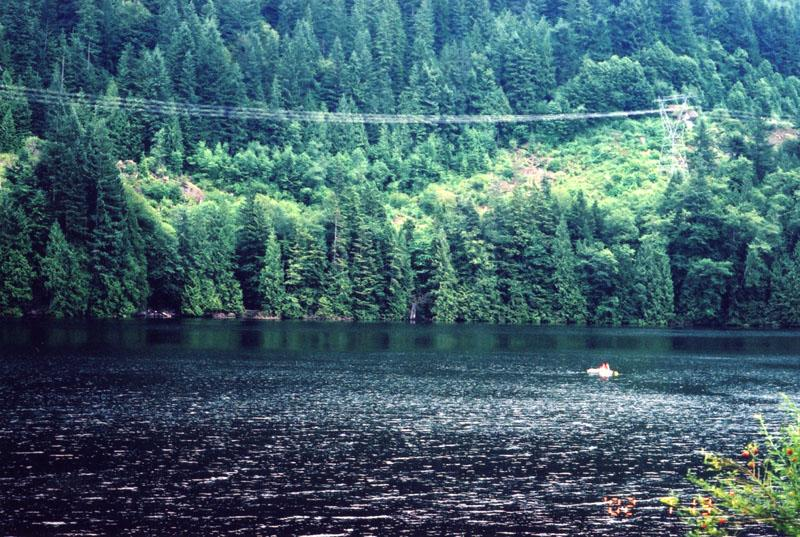
\includegraphics[width=0.4\textwidth]{lake1}
\caption{Text wrap around figure}
\noindent \hrulefill
\label{test}
\end{wrapfigure}
\end{verbatim}

\end{itemize}

\foilhead[-0.8in]{}
\MyLogo{The text in this slide is from 
\href{http://www.ctan.org/tex-archive/macros/latex/contrib/supported/wrapfig/wrapfig.sty}{wrapfig manual}.}    %make a left footer
 Wrapfig.sty provides the environments ``wrapfigure'' and ``wraptable'' for 
typesetting a narrow float at the edge of the text, and making the text wrap 
around it. The ``wrapfigure'' and ``wraptable'' environments interact properly 
with the \verb+\caption+ command to produce proper numbering, but they are not 
regular floats like ``figure'' and ``table'', so (beware!) they may be printed 
out of sequence with the regular floats. There are four parameters 
for \verb+\begin{wrapfigure}+, two optional and 
\begin{wrapfigure}{r}{0.4\textwidth}
\renewcommand{\captionfont}{\small \bfseries \sffamily}
\centering
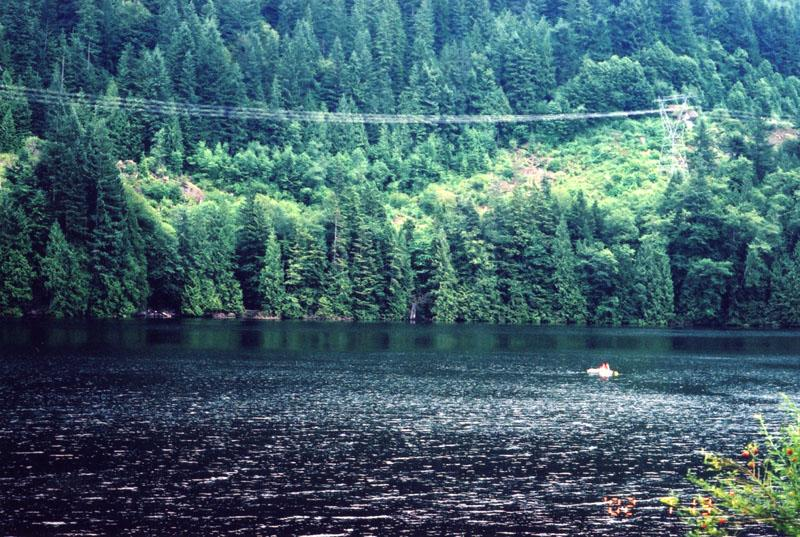
\includegraphics[width=0.3\textwidth]{lake1}
\caption{Text wrap around figure}
\noindent \hrulefill
\label{test}
\end{wrapfigure}
two required, plus the text of 
the figure, with a caption perhaps.
You must not specify a wrapfigure in any type of list environment or or 
immediately before or immediately after one. It is OK to follow a list if 
there is a blank line (\verb+\par+) in between.
If you put a wrapfigure in a parbox or a minipage, or any other type of grouping, the text wrapping should end before the group does.
It does work in two-column format, but are your figures that small?
It may be out of sequence with regular floats.
The hlines that may be printed above and below floats are ignored; 
you must insert them manually if desired.
\verb+\linewidth+ is not adjusted within the wrapped text (because it can only be set for whole paragraphs at a time). It is set within the figure.



\foilhead[-0.8in]{}
\MyLogo{Eugenia and Weiliang, UBC Stats}    %make a left footer

\bibliographystyle{plain}
\bibliography{workshop}


\end{document}
